\section{Introduction}
\label{sec:intro}

Reward models for language-model alignment, rating systems for games, and
recommenders trained on clicks all learn from the same kind of data: pairs.
Response $B$ was preferred to response $A$; player $j$ beat player $i$. A set
of such comparisons lives on the edges of a \emph{comparison graph}, and
combinatorial Hodge theory \cite{jiang2011statistical} splits every edge flow
orthogonally into three parts (Figure~\ref{fig:schematic}): a
\emph{gradient} part, the differences of a global score --- a ranking; a
\emph{curl} part, circulation around triangles --- rock--paper--scissors; and a
\emph{harmonic} part, circulation around larger holes of the graph. A scalar
reward model, the Bradley--Terry workhorse of RLHF \cite{bradley1952rank,
ouyang2022training}, can only express the first. Skew-symmetric models such as
the General Preference Model (GPM) \cite{zhang2025beyond} and hybrid
reward--cyclic decompositions \cite{hrc2026transitivity} were proposed
precisely to capture the other two.

\begin{figure}[t]
\centering
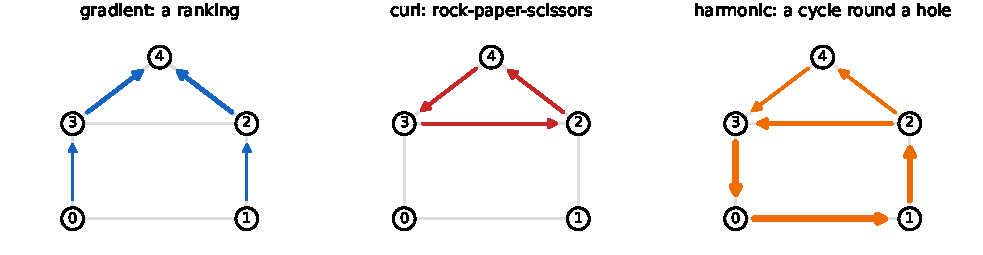
\includegraphics[width=\columnwidth]{figures/schematic.pdf}
\caption{The three Hodge components of one edge flow on a five-item
comparison graph (triangle 2--3--4 filled): a ranking, a local cycle, and a
cycle around the square hole. Arrow width is flow magnitude.}
\label{fig:schematic}
\end{figure}

That literature asks what a model \emph{can} represent. We ask what gradient
descent \emph{learns first}. The question has teeth. If a flexible preference
model fits the ranking long before it fits the cycles, then (i) the number of
training steps is an implicit prior on transitivity; (ii) early stopping acts
as a transitivity filter, discarding cyclic structure whether it is real or
noise; and (iii) since random label noise on a well-connected graph falls
almost entirely in cycle space, that filter should be most useful exactly when
annotators disagree. The neural tangent kernel \cite{jacot2018neural} is the
natural tool: in the linearised regime \cite{lee2019wide}, gradient descent
fits each eigen-direction of the kernel at a rate set by its eigenvalue, and
the infinite-width limit is a Gaussian process \cite{neal1996bayesian,
lee2018deep} --- here a GP preference model \cite{chu2005preference} with a
specific, computable kernel. What is missing is the kernel \emph{between
edges} and its relation to the Hodge subspaces.

We compute that kernel for three models, in closed form at infinite width and
empirically at finite width, and test four hypotheses: that the scalar
kernel is blind to cycles (H0); that the antisymmetric kernel is spectrally
ordered, gradient first (H1); that training follows that order (H2); and that
noise is cyclic and early stopping filters it (H3). We then test the whole
picture on \AreVotes\ human votes from Chatbot Arena (H4). H0--H2 hold
cleanly; parts of H1 and H3 do not, and we report where and why.
